\chapter{Methodology}

This chapter describes how the raw data become model inputs and how the models are evaluated.
Figure~\ref{fig:pipeline} gives an overview. Ground \pmtf{} passes through quality control; all
data are then aligned to IST days (or hours, for forecasting), turned into features and passed to
the models, which are evaluated under several validation schemes.

\begin{figure}[!htbp]
\centering
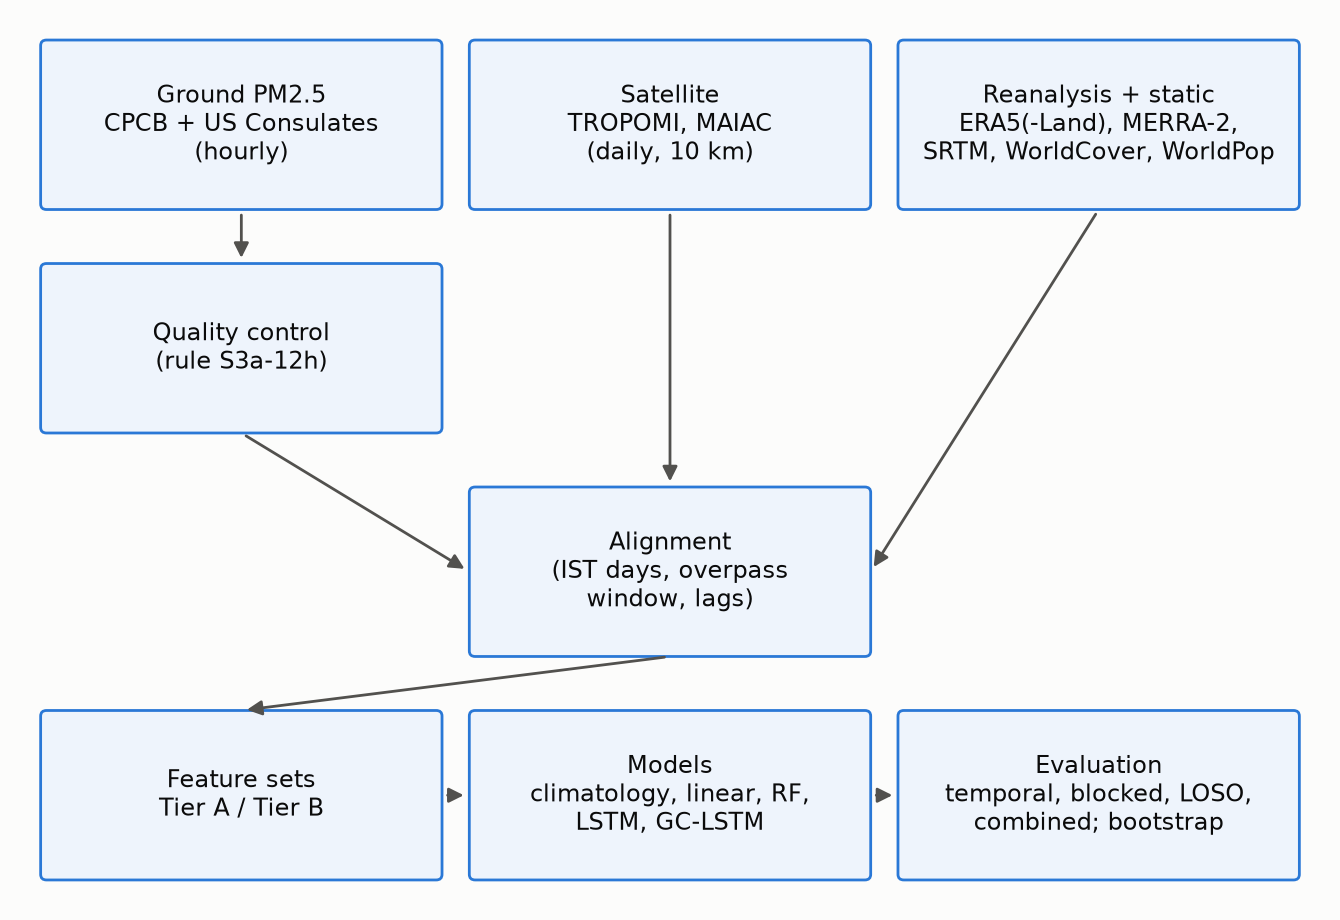
\includegraphics[width=0.8\linewidth]{thesis_pipeline}
\caption{Processing pipeline of the study.}
\label{fig:pipeline}
\end{figure}

\section{Reproducibility}

The pipeline is a set of small Python scripts run through one entry point, with every setting in
YAML configuration files, pinned package versions and a fixed random seed (42). Each raw file is
recorded in the data manifest with its SHA-256 hash. Every removal of data is logged with a reason,
and row counts are reconciled from raw hours to the final dataset. Each methodological decision,
with the alternatives considered, is recorded in a decision log, and the tests check the
time conversions, the quality-control rules and the absence of leakage between training and
test data.

\section{Quality control}

Quality control is applied to the hourly ground data. No row is deleted: each hour receives a flag,
and only hours flagged as valid enter the daily targets. Algorithm~\ref{alg:qc} lists the rule,
named S3a-12h in the decision log, and Table~\ref{tab:qc} its effect.

\begin{algorithm}[!htbp]
	\caption{Hourly \pmtf{} quality control (rule S3a-12h)}
	\label{alg:qc}
	\begin{algorithmic}[1]
		\STATE \textbf{Input}: hourly series $x_t$ of one station
		\FOR{each hour $t$}
			\IF{$x_t < 0$, or $x_t = 0$, or $x_t = 1000$\ugm{}}
				\STATE flag $t$ as invalid
			\ENDIF
		\ENDFOR
		\STATE flag every run of identical values lasting at least 12 consecutive hours as a flat line
		\STATE $m_t \leftarrow$ median of $x$ over the centred 25-hour window around $t$
		\STATE flag runs of 1--2 hours with $x_t > 4\,m_t$ and $x_t > 100$\ugm{} as isolated spikes
		\STATE \textbf{Output}: a flag for every hour; only unflagged hours are used
	\end{algorithmic}
\end{algorithm}

\begin{table}[!htbp]
    \centering
    \small
    \begin{tabular}{l|r}
        \hline
        Rule & Hours removed \\
        \hline
        Negative / zero / exactly 1000\ugm{} & 17 / 39 / 2 \\
        Flat run of 12 hours or more & 16,334 \\
        Isolated spike & 3,880 \\
        \hline
        Total & 20,272 of 2,965,479 (0.68\,\%) \\
        \hline
    \end{tabular}
    \caption{Effect of the quality-control rule on the hourly ground data.}
    \label{tab:qc}
\end{table}

Hours above 500\ugm{} that are neither spikes nor flat lines are kept, because events such as
festival fireworks are real. The flat-line threshold was first set at 24 hours. It was lowered to
12 hours after a sensitivity run showed that runs of 12--23 identical hourly values look like stuck
instruments: round values such as 45.0 repeated 379 times, and values above 100\ugm{} three and a
half times more common than elsewhere. Because this change was made after its effect on model
skill had been seen, the results under the 24-hour rule are reported alongside the main results
(Section~\ref{sec:sensitivity}).

\section{Targets and temporal alignment}\label{sec:align}

The primary target is the daily mean \pmtf{} of an IST calendar day, valid when at least 18 of the
24 hourly values pass quality control. A secondary target, the mean of the three hours starting at
12:00--14:00 IST (valid with at least two of the three), matches the TROPOMI and MODIS Aqua overpass
times and is used in a sensitivity test.

All raw timestamps are converted from UTC to IST before aggregation. Hourly meteorology is averaged
over each IST day (precipitation is summed). Relative humidity is computed from 2\,m temperature $T$
and dew point $T_d$ (both in \textdegree C) with the Magnus formula:
\begin{equation}\label{eq:rh}
\mathrm{RH} = 100\,\frac{\exp\!\left(\frac{17.625\,T_d}{243.04 + T_d}\right)}{\exp\!\left(\frac{17.625\,T}{243.04 + T}\right)}.
\end{equation}
MERRA-2 surface \pmtf{} is reconstructed from the dust, organic carbon, black carbon, sea salt and
sulphate surface mass concentrations, with sulphate converted to ammonium sulphate:
\begin{equation}\label{eq:merra2}
\mathrm{PM}_{2.5}^{\mathrm{M2}} = \mathrm{DU}_{2.5} + \mathrm{OC} + \mathrm{BC} + \mathrm{SS}_{2.5} + \frac{132.14}{96.06}\,\mathrm{SO_4}.
\end{equation}

The final dataset has 126,805 station-days at 113 stations, of which 113,228 have a valid daily
target and 124,102 a valid overpass target.

\section{Features and the two-tier model}

Table~\ref{tab:features} lists the feature groups. Lags are calendar lags: the value on the
previous calendar day, left missing if that day is absent, never the previous available row.
Missing satellite values stay missing; the Random Forest handles them natively, and the linear
model replaces them with medians computed on the training rows.

\begin{table}[!htbp]
    \centering
    \small
    \begin{tabular}{L{2.8cm}|L{7.4cm}|c}
        \hline
        Group & Variables & Tier \\
        \hline
        Satellite & TROPOMI NO\textsubscript{2}, CO, SO\textsubscript{2}, HCHO, UV aerosol index, cloud fraction; MAIAC AOD; valid-pixel counts and availability flags (10 km) & A \\
        Reanalysis aerosol & MERRA-2 \pmtf{} and AOD & A, B \\
        Meteorology & Temperature, relative humidity, wind components and speed, precipitation, boundary-layer height & A, B \\
        Lags & \pmtf{} 1--3 days; meteorology 1 day; precipitation 2--3 days & A, B \\
        Temporal & Day of year (sine and cosine), month, season & A, B \\
        Static & Elevation, distance to coast, land-cover shares, population & A, B \\
        \hline
    \end{tabular}
    \caption{Feature groups. Tier A has 43 features and Tier B 31.}
    \label{tab:features}
\end{table}

Tier A is trained and evaluated only on station-days where MAIAC AOD exists within 10\,km; Tier B
is trained on all station-days. The two-tier prediction uses Tier A where it applies and Tier B
otherwise. To isolate the effect of the satellite inputs, Tier B is also scored on exactly the
station-days where Tier A applies.

Each tier is run with and without the \pmtf{} lags. The versions with lags need yesterday's
measurement at the same station, so they describe gap filling at a monitored site. The versions
without lags are the relevant measure for unmonitored locations.

\section{Validation design}

Table~\ref{tab:splits} lists the four validation schemes. Spatial blocks are formed by linking
stations that lie within 50\,km of each other (single linkage), so that a city's cluster of stations
always falls on the same side of a split. This gives 46 blocks, which are assigned to five folds
with balanced numbers of rows.

\begin{table}[!htbp]
    \centering
    \small
    \setlength{\tabcolsep}{4pt}
    \begin{tabular}{l|l|l}
        \hline
        Split & Training data & Test data \\
        \hline
        Temporal & 2021--2024 & 2025 \\
        Spatially blocked & four of five folds of blocks & the fifth fold \\
        Leave-one-station-out (LOSO) & all other stations & one station \\
        Combined & other blocks, 2021--2024 & held-out blocks, 2025 \\
        \hline
    \end{tabular}
    \caption{Validation schemes.}
    \label{tab:splits}
\end{table}

Four models are compared. Persistence predicts yesterday's value at the same station (temporal
split only). Climatology predicts the training mean for the station and calendar month, falling
back to the state and month for an unseen station. Linear regression uses median-imputed,
standardised features. The Random Forest \cite{breiman2001rf} uses fixed settings: 200 trees,
a minimum of five samples per leaf, half of the features considered at each split and half of the
rows drawn for each tree. All preprocessing is fitted on the training rows only. The models were
implemented with scikit-learn \cite{pedregosa2011sklearn}.

Skill is measured on the pooled held-out rows with the coefficient of determination, the root mean
square error (RMSE) and the mean absolute error:
\begin{equation}\label{eq:r2}
R^2 = 1 - \frac{\sum_i (y_i - \hat{y}_i)^2}{\sum_i (y_i - \bar{y})^2}, \qquad
\mathrm{RMSE} = \sqrt{\frac{1}{n}\sum_i (y_i - \hat{y}_i)^2},
\end{equation}
where $y_i$ is the observed and $\hat{y}_i$ the predicted value. Results are broken down by season,
by TROPOMI cloud fraction (0--0.2, 0.2--0.5, 0.5--0.8 and 0.8--1.0), by station and for Kerala in
June--September.

Errors are correlated within a city and across neighbouring days, so resampling individual rows
would give intervals that are far too narrow. Confidence intervals are therefore percentile
intervals from 1,000 bootstrap resamples of the 46 spatial blocks \cite{efron1993bootstrap}, each
drawn block contributing all of its rows. Differences between two models are bootstrapped on the
same rows (a paired bootstrap).

\section{Hourly forecasting at existing stations}\label{sec:method_forecast}

As an extension, \pmtf{} is forecast 1 to 72 hours ahead at the 113 stations, the task addressed by
the forecasting studies in Chapter~2. A forecast is issued at the end of each IST hour $H$, once that
hour's measurement is available, and targets the quality-controlled hourly value at $H + h$.
Results are reported at $h$ = 1, 3, 6, 12, 24, 48 and 72 hours. Every input is restricted to what is
known at the issue time (Table~\ref{tab:fc_inputs}).

\begin{table}[!htbp]
    \centering
    \small
    \begin{tabular}{L{4.6cm}|L{3.2cm}|L{3.8cm}}
        \hline
        Input & Setting (a): past only & Setting (b): + weather ahead \\
        \hline
        \pmtf{} at the station (and neighbours, graph model) & hours $\le H$ & same \\
        ERA5 instantaneous fields & hours $\le H$ & also at the target hours \\
        Precipitation, MERRA-2 (hourly averages) & hours $\le H-1$ & precipitation also at the target hours \\
        Satellite (daily) & day $d$ if $H \ge$ 15 IST, else $d-1$ & same \\
        Calendar of the target hour; static features & yes & yes \\
        \hline
    \end{tabular}
    \caption{Information available to a forecast issued at hour $H$.}
    \label{tab:fc_inputs}
\end{table}

ERA5 instantaneous values are stamped on the UTC hour, which is half past the hour in IST, so they
fall inside the IST hour they describe. Hourly averages and accumulations may extend past the issue
time, so they are used only up to $H-1$. Satellite values for a day are used only from 15:00 IST,
after the MODIS Aqua granules over the region end. Setting (b) adds reanalysis weather for the
target hours and is an upper bound: it assumes a perfect weather forecast. Training uses issue
hours in 2021--2023, the validation year 2024 is used only for early stopping and tuning of the
neural networks, and 2025 is the test year. The last 72 hours of the training and validation
periods are dropped so that no target falls in the next period.

\subsection{Tabular models}

Persistence uses the last valid value within 24 hours. Climatology uses the training mean for the
station, month and hour of day. Linear regression and the Random Forest (settings as above, trained
on a random third of the training rows to limit cost) are fitted separately for each horizon on
issue-time features: \pmtf{} at lags of 0, 1, 2, 3, 6, 12, 23, 24 and 48 hours, means and valid
counts over the last 6, 24 and 72 hours, the last valid value and its age, current meteorology and
its 24-hour mean, lagged precipitation and MERRA-2, the calendar of the target hour and the static
features.

\subsection{LSTM and graph network}

The LSTM \cite{hochreiter1997lstm} reads the past 72 hours of each station's inputs, $x_1, \ldots,
x_{72}$, and updates a hidden state $h_t$ and a cell state $c_t$ through input, forget and output
gates:
\begin{equation}\label{eq:lstm}
\begin{aligned}
i_t &= \sigma(W_i x_t + U_i h_{t-1} + b_i), \qquad f_t = \sigma(W_f x_t + U_f h_{t-1} + b_f),\\
o_t &= \sigma(W_o x_t + U_o h_{t-1} + b_o), \qquad h_t = o_t \odot \tanh(c_t),\\
c_t &= f_t \odot c_{t-1} + i_t \odot \tanh(W_c x_t + U_c h_{t-1} + b_c).
\end{aligned}
\end{equation}
A feed-forward head combines the final hidden state with the station's static features, the
calendar of each target hour, a learned embedding of the horizon and, in setting (b), the weather
at the target hour, and outputs all 72 horizons at once. The head predicts the change from the
station's latest \pmtf{} value rather than the value itself.

The graph network follows the GC-LSTM of Qi et al.\ \cite{qi2019gclstm}. At every time step a graph
convolution \cite{kipf2017gcn} mixes each station's inputs with those of its neighbours before the
LSTM. Stations within 200\,km are linked (median 19 neighbours), with weights that decrease with
distance $d_{ij}$, and the adjacency matrix is normalised symmetrically:
\begin{equation}\label{eq:gcn}
w_{ij} = \exp\!\left[-\left(\frac{d_{ij}}{100\,\mathrm{km}}\right)^{2}\right] \ \text{for}\ d_{ij} \le 200\,\mathrm{km}, \qquad
\hat{A} = D^{-1/2}(W + I)\,D^{-1/2},
\end{equation}
where $D$ is the diagonal degree matrix of $W + I$.

Missing \pmtf{} inputs are carried forward for up to 24 hours, otherwise replaced by the station's
training median, and a second input channel marks which values were observed. All inputs are
standardised with training statistics, and the loss is the mean squared error on observed targets
only. Both networks have 64 hidden units and are trained with Adam (learning rate 0.001) on batches
of 16 issue hours, each containing all stations; every epoch uses a random third of the training
issue hours, and training stops when the validation loss has not improved for eight epochs. Each
configuration is trained with three seeds. The networks were implemented in PyTorch
\cite{paszke2019pytorch}.

Five settings were compared on the validation year only (the base settings, a lower learning rate,
weight decay with more dropout, 128 hidden units and a 24-hour input window). Their mean validation
\rsq{} over the reported horizons ranged from 0.495 to 0.499, so the base settings were kept. The
change to predicting the difference from the latest value was made after the first LSTM run scored
below persistence at short horizons on the test year; this is the only choice informed by the test
year.

As in the estimation task, Tier A adds the latest satellite day's features and is evaluated where
that day has MAIAC AOD; Tier B uses no satellite input. Confidence intervals come from a paired
bootstrap over spatial block $\times$ calendar month of the test year (about 500 clusters), because
forecast errors are strongly correlated in time.
